\documentclass{beamer}
\usetheme{Zurich}
\usepackage{amsmath, amsfonts, graphicx, multirow}
\title{Boosting}
\author{Charlotte Wickham}
\date{\today}

\begin{document}

\frame{\titlepage}

\begin{frame}
	\frametitle{Boosting}
	Idea in the binary classification context ($Y \in \{-1,1\}$).
	\begin{itemize}
		\item Take a weak classifier (one that does just a bit better than random guessing).
		\item Fit the classifier to the data to get $G_1(X)$.
		\item Give more weight to the observations in the training set it gets wrong.
		\item Re-fit the classifier to the reweighted data.
		\item Repeat M times to get a sequence of classifiers, $G_m(X)$.
		\item The predicted value of a new data point is a \textbf{weighted} sum of classifiers. 
		\[
		G(x) = \text{sign} \left( \sum_{m=1}^M{\alpha_m G_m(x)} \right)
		\]
	\end{itemize}
\end{frame}

\begin{frame}
	Choices:
	\begin{itemize}
		\item How are the observations reweighted?
		\item How are the classifiers weighted in the prediction?
		\item What weak classifier to use?
	\end{itemize}
\end{frame}

\begin{frame}
	\frametitle{AdaBoost Algorithm}
	\begin{enumerate}
		\item Initialize weights, $w_i = 1/N$ for $i = 1,\ldots, N$
		\item For $m=1$ to $M$
		\begin{enumerate}
			\item Fit classifier to the training data using weight $w_i$ to get $G_m(x)$.
			\item Calculate the the training set error
			\[
			\text{error}_m = \frac{\sum_{i=1}^N w_i I(y_i \ne G_m(x_i))}{\sum_{i=1}^N w_i}
			\]
			\item Calculate
			\[
			\alpha_m = \log{\frac{1 - \text{error}_m}{\text{error}_m}}
			\]
			\item Set $w_i \leftarrow  w_i \exp(\alpha_m I(y_i \ne G_m(x_i)))$ for $i=1,\ldots, N$
			\end{enumerate}	
		\item Output $G(x) = \text{sign} \left( \sum_{m=1}^M{\alpha_m G_m(x)} \right)$	
	\end{enumerate}
\end{frame}


\begin{frame}
\frametitle{AdaBoost Algorithm}
\begin{columns}[c] 
	\column{.4\textwidth} 
		\setkeys{Gin}{width=\textwidth}
		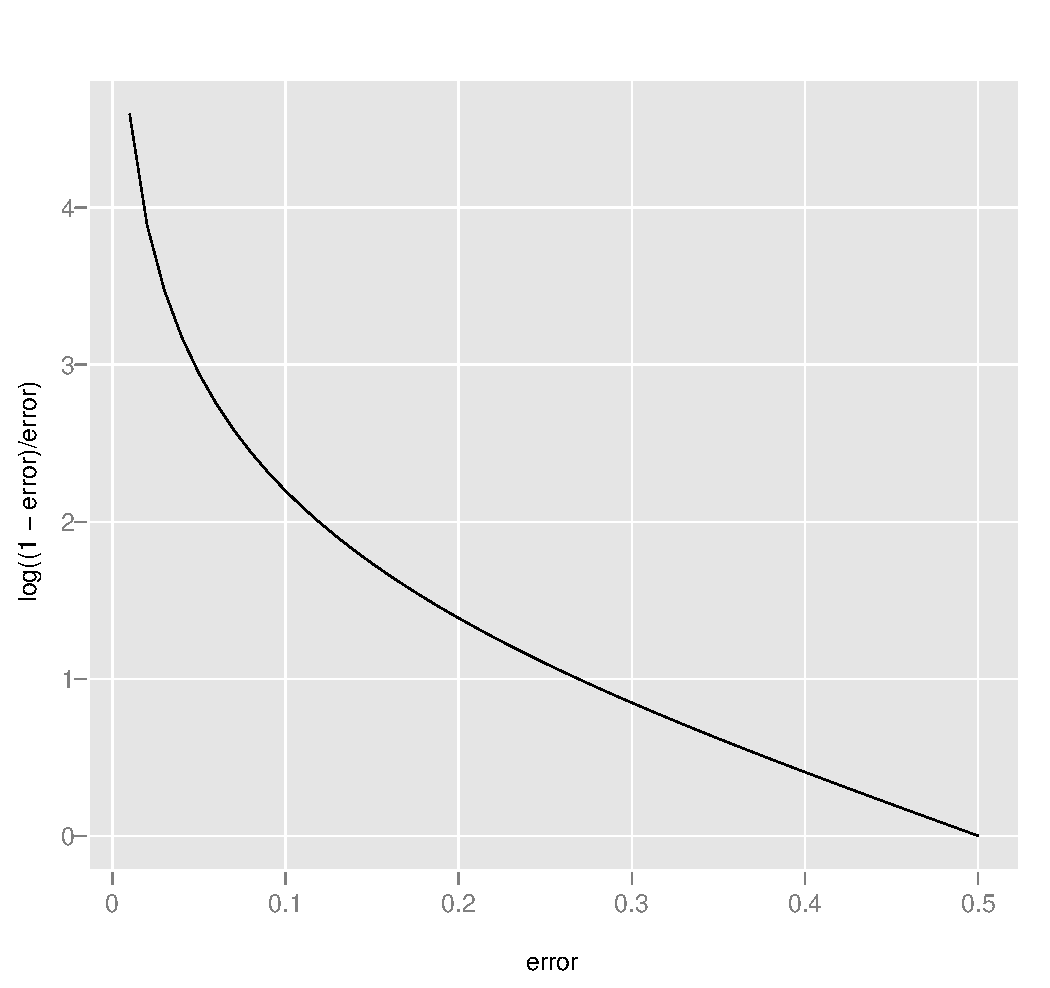
\includegraphics{log.pdf}\\
		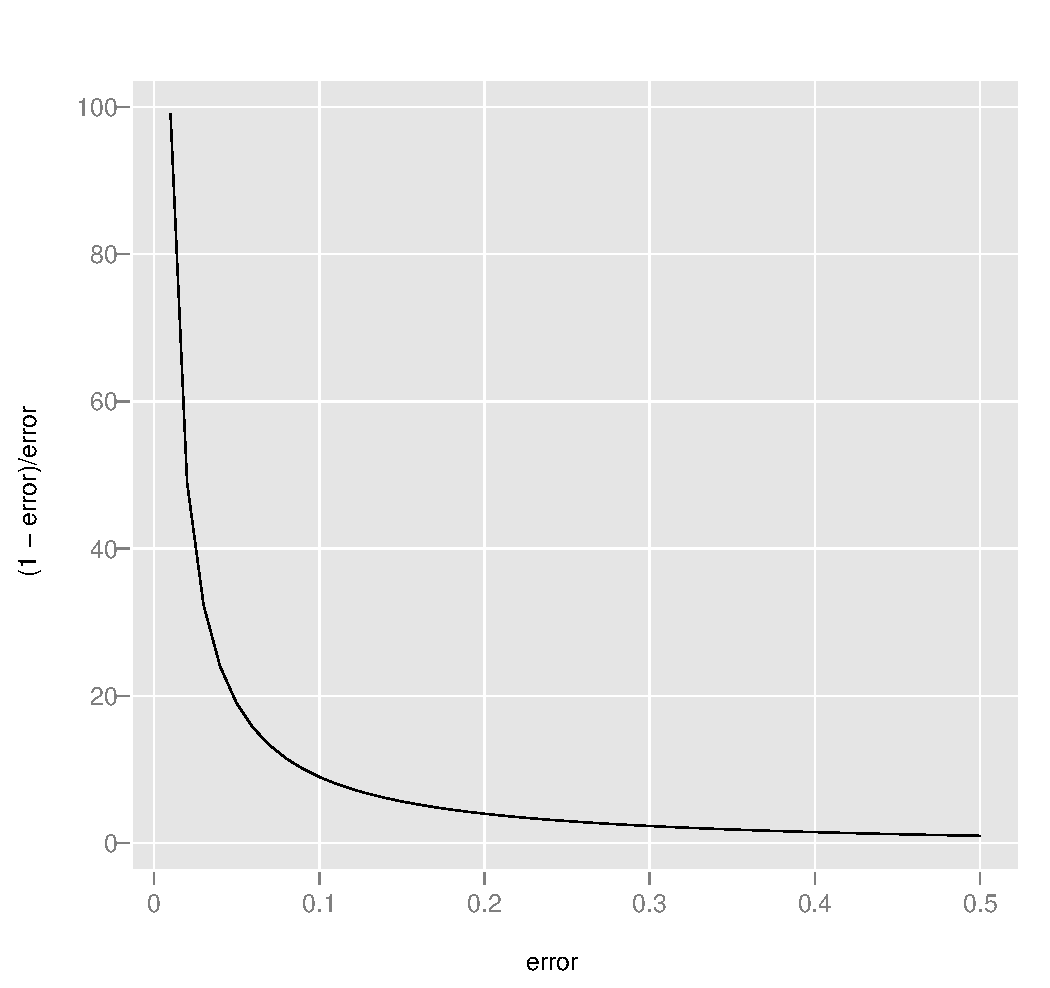
\includegraphics{exp.pdf}
	\column{.6\textwidth}
	\begin{itemize}
		\item Gives more weight to classifiers in the sequence with low training error.	
		\item Gives more weight to observations that are misclassified.  The better the classifier overall the bigger the weight on the misclassified observations.
		\item Choice of classifier is free. Often use trees with very few splits.  Stump = tree with one split.
	\end{itemize}
	\end{columns}
\end{frame}
\begin{frame}
	\frametitle{Performance on test set}
	\begin{itemize}
		\item Trees with one split (stumps)
		\begin{table}
		\begin{tabular}{cr|rr}
		& & \multicolumn{2}{c}{Prediction}\\
		& & Other & Supernova\\
		\hline
		\multirow{2}{*}{\rotatebox{90}{Actual}} & Other &  451 &  49\\
		& Supernova & 47 &  453\\
		\end{tabular}
		\end{table}
		Error: 9.6\%
		\setkeys{Gin}{width = 0.8\textwidth}
		\begin{figure}
		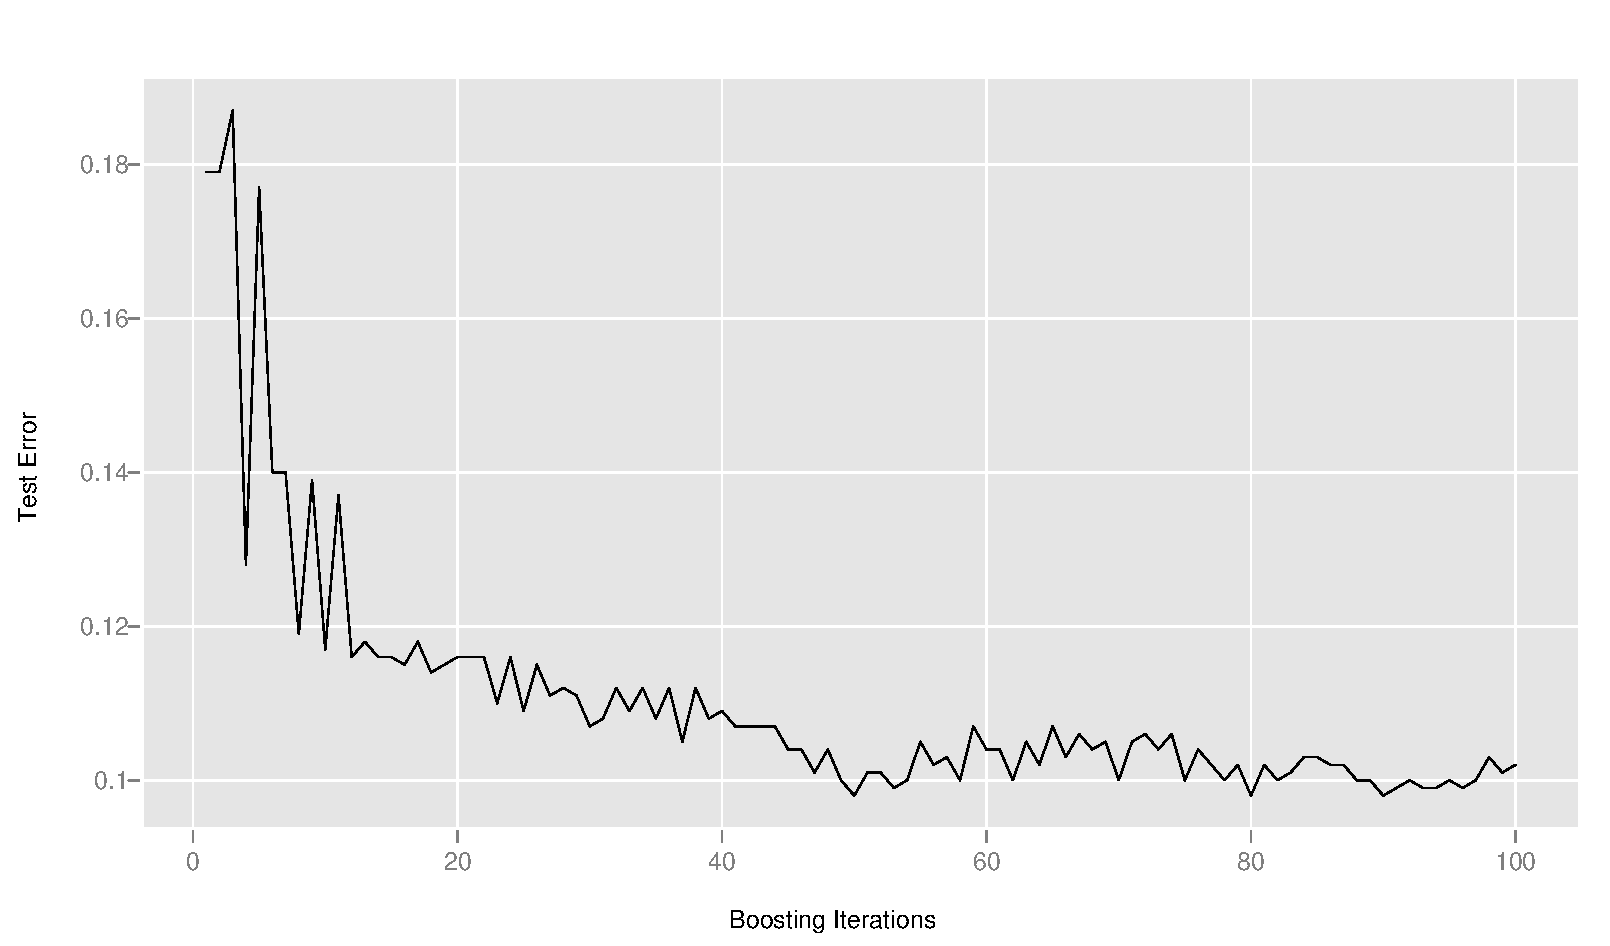
\includegraphics{error.pdf}
		\end{figure}
			\end{itemize}

\end{frame}

\begin{frame}
		Got about 8\% from CART and 6\% from bagging and 5\% from random forests.
		\begin{itemize}
			\item Trees with two splits
			\begin{table}
			\begin{tabular}{cr|rr}
			& & \multicolumn{2}{c}{Prediction}\\
			& & Other & Supernova\\
			\hline
			\multirow{2}{*}{\rotatebox{90}{Actual}} & Other &  455 &  45\\
			& Supernova & 45 &  455\\
			\end{tabular}
			\end{table}
			Error: 9.0\%
			
			\item Trees with three splits
			\begin{table}
			\begin{tabular}{cr|rr}
			& & \multicolumn{2}{c}{Prediction}\\
			& & Other & Supernova\\
			\hline
			\multirow{2}{*}{\rotatebox{90}{Actual}} & Other &  455 &  45\\
			& Supernova & 47 &  453\\
			\end{tabular}
			\end{table}
			Error: 9.2\%
		\end{itemize}
\end{frame}




\begin{frame}
	\frametitle{More general idea}
	Our output is
	\[
	G(x) = \text{sign} \left( \sum_{m=1}^M{\alpha_m G_m(x)} \right)
	\]
	Imagine we knew $G_m(x)$ and $\alpha_m$ for $m = 1,\ldots, M-1$ and let their contribution to the output be $g_{M-1}$.  Then we could imagine searching for the optimal $G_M$ and $\alpha_M$ that would minimize our error according to some loss function.  I.e. find $G_M$ and $\alpha_M$
	\[
	(G_m, \alpha_M) = \arg \min_{G_m, \alpha_M}\sum_{i=1}^N \mathcal{L}\left(y_i, g_{M-1}(x) + \alpha_m G_m(x)\right)
	\]
\end{frame}

\begin{frame}
	\frametitle{More general idea}
	\begin{itemize}
		\item We could envisage a stagewise process where we begin with a base model and then iteratively add terms by the minimization presented.
		\item In fact, AdaBoost is equivalent to this process if you use the loss function,
		\[
		\mathcal{L}(y, G(x)) = \exp(-y G(x)).
		\] 
		\item Why use this loss?
			\begin{itemize}
				\item Computationally easy
			\end{itemize}
		\item There are other possibilities but they require more effort in the minimization step.
	\end{itemize}
\end{frame}

\begin{frame}
	\frametitle{Gradient Boosting with trees}
	We want to solve,
		\[
		\arg \min_{\Theta_m}\sum_{i=1}^N\mathcal{L}(y_i, g_{m-1}(x_i) + T(x_i; \Theta_m))
		\]
		where $\Theta_m = \{R_{jm}, \phi_{jm}\}_1^{J_m}$ is the region sets and constants for the tree.
	
	\begin{itemize}
		\item For complicated loss functions this can be really hard.
		\item We want a way to approximate this minimisation.
		\item In general how do we minimise things: 
			gradient descent
	\end{itemize}
	
\end{frame}

\begin{frame}
	\frametitle{Steepest descent}
	Say we want to find $\hat{G} = \arg \min_G \mathcal{L}(G)$ where $\mathcal{L}(G) = \sum_{i=1}^N \mathcal{L}(y_i, G(x_i))$.

 At each iteration we take a step in the direction that most minimizes our error. The components of this gradient, $h_m$ are:
	\[
	h_{im} = \left[ \frac{\delta \mathcal{L}(y_i, G(x_i))}{\delta G(x_i)}\right]_{G(x_i) = g_{m-1}(x_i)}
	\]
 and the step length, $\rho_m$, is the solution to
	\[
	 \rho_m = \arg \min_\rho \mathcal{L}(g_{m-1} - \rho h_m).
	\]	
Then the updated solution is
\[
g_m = g_{m-1} - \rho_m h_m
\]	

\end{frame}

\begin{frame}
	\frametitle{Gradient Boosting}
	So the stepwise procedure outlined earlier is a lot like steepest descent where the new tree is analogous to the components of the negative gradient.
\begin{itemize}
	\item{Problems}
		\[
		\arg \min_{\Theta_m}\sum_{i=1}^N\mathcal{L}(y_i, g_{m-1}(x_i) + T(x_i; \Theta_m))
		\]
	is hard to calculate for robust losses.  We would like to use the gradient descent method instead since,
	\[
	h_{im} = \left[ \frac{\delta \mathcal{L}(y_i, G(x_i))}{\delta G(x_i)}\right]_{G(x_i) = g_{m-1}(x_i)}
	\]
 is easy to calculate for most loss functions. However,	it is  only defined at $x_i$ and eventually we want to generalize to new cases.
\end{itemize}

\end{frame}

\begin{frame}
	\frametitle{Gradient Boosting}
	Possible resolution
	\begin{itemize}
		\item 
		Induce a tree at the $m^{th}$ iteration that approximates the negative gradient
		\[
		\tilde{\Theta}_m = \arg \min_\Theta \sum_{i=1}^N (-h_{im} - T(x_i; \Theta))^2
		\]
		\item This is just a normal regression tree and there are good algorithms for finding it.
		
		\item the constants for each region ($\gamma_{jm}$) are then found from
		\[
		\gamma_{jm} = \arg \min_{\gamma_{jm}} \sum_{x_i \in R_{jm}} \mathcal{L}(y_i, g_{m-1}(x_i) + \gamma_{jm}) 
		\]
	\end{itemize}
Leads to the MART algorithm
	
\end{frame}

\begin{frame}
	\frametitle{MART for regression}
	\begin{enumerate}
		\item Initialize $g_0(x) = \arg \min_\gamma \sum_{i=1}^N \mathcal{L}(y_i, \gamma)$
		\item for $m=1$ to M
		\begin{enumerate}
			\item For $i=1,2,\ldots, N$ compute
			\[
			r_{im} = - \left[ \frac{\delta \mathcal{L}(y_i, G(x_i))}{\delta G(x_i)}\right]_{G(x_i) = g_{m-1}(x_i)}
			\]
		\item Fit a regression tree to the target $r_{jm}$ giving terminal regions $R_{jm}$, $j = 1,2,\ldots, J_m$.
		\item For $j = 1,2,\ldots, J_m$ compute 
			\[
			\gamma_{jm} = \arg \min_{\gamma} \sum_{x_i \in R_{jm}} \mathcal{L}(y_i, g_{m-1}(x_i) + \gamma) 
			\]
		\item Update $g_m = g_{m-1} + \sum_{j=1}^{J_m} \gamma_{jm}I(x \in R_{jm}) $
		\end{enumerate}
	\item{Output $\hat{f}(x) = f_M(x)$}
	\end{enumerate}
\end{frame}

\begin{frame}
	\frametitle{MART}
\begin{itemize}
	\item Extends to classification by repeating steps for each class K.
	\item Tuning parameters are the size of the trees $J_m$ and the number of iterations M.
	\item In practice choose $J_m = J$ between 4 and 8.
	\item Choose M based on cross validation or a separate training set.  

\end{itemize}
\end{frame}



\end{document}